\chapter{Agenti Intelligenti}

\begin{definition-box}{Agente}
Un \textbf{agente} è qualsiasi cosa che può percepire il suo ambiente
tramite dei \textbf{sensori} e che può agire sul suo ambiente
tramite degli \textbf{attuatori}.
\end{definition-box}

Un agente elabora le percezioni che ha sull'ambiente e ne deriva le azioni da
eseguire per ottenere lo stato desiderato.

La storia completa di tutto ciò che l'agente ha percepito è detta
\textbf{sequenza di percezione}.

L'azione di un agente in un determinato momento dipende dalla sua conoscenza e
dalla sua sequenza di percezione osservata fino a quel momento.

Matematicamente possiamo dire che il comportamento di un agente è descritto
dalla \textbf{funzione agente} che mappa ogni possibile sequenza percettiva a
un'azione.

Potremmo pensare di realizzare una tabella che associa a ogni possibile
sequenza percettiva l'azione che l'utente deve compiere ed essa rappresenterebbe
un'implementazione della funzione agente.

La funzione agente è solo una rappresentazione matematica astratta,
internamente essa sarà implementata come \textbf{programma agente}.

\begin{figure}[H]
	\centering
	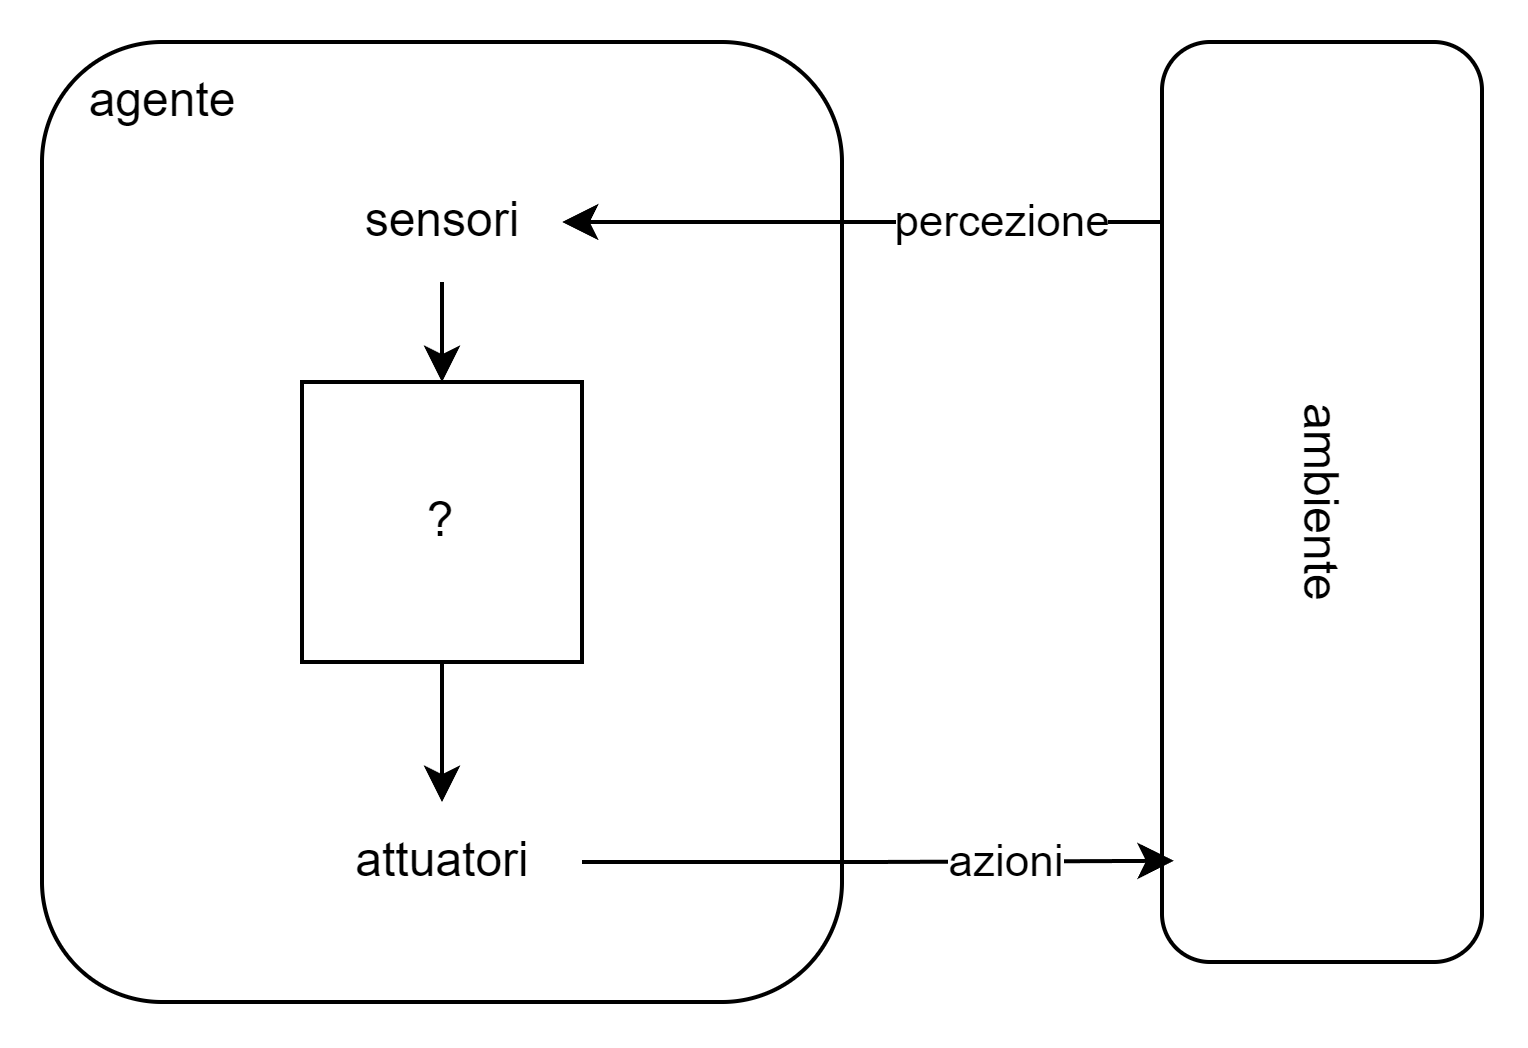
\includegraphics[width=0.8\textwidth]{capitoli/agenti-intelligenti/imgs/agente.png}
\end{figure}

\section{Concetto di Razionalità}

\begin{definition-box}{Agente razionale}
Un \textbf{agente razionale} è un agente che fa la cosa giusta.
\end{definition-box}

Per valutare cosa significa fare la cosa giusta utilizziamo la nozione del
\textbf{consequenzialità}: valutiamo il comportamento di un agente dalle sue
conseguenze.

Nel momento in cui un agente è a contatto con un ambiente, genererà una serie
di azioni che faranno passare l'ambiente in una sequenza di stati. Se tale
sequenza è \textbf{desiderabile} allora l'agente si è comportato bene.

La desiderabilità di una sequenza di stati è valutata dalla
\textbf{misurazione delle performance}.

Ciò che è razionale in un dato istante dipende da:

\begin{itemize}
	\item La misura delle performance che definisce il criterio di successo.
	\item La conoscenza pregressa che l'agente ha dell'ambiente.
	\item Le azioni che l'agente può svolgere.
	\item La sequenza percettiva fino a quel momento.
\end{itemize}

\begin{definition-box}{Agente razionale}
Un \textbf{agente razionale} deve selezionare un'azione che ci si aspetta
massimizzi la misurazione delle performance, data l'evidenza fornita dalla
sequenza percettiva e dalla conoscenza dell'agente.
\end{definition-box}

\section{Natura degli Ambienti}

Prima di poter pensare a come costruire un agente dobbiamo studiare gli
\textbf{ambienti di lavoro}, che sono i problemi per i quali gli agenti sono la
soluzione. La natura dell'ambiente di lavoro influenza direttamente il design
appropriato per l'agente.

L'ambiente di lavoro è composto da quattro componenti principali:

\begin{itemize}
	\item \textbf{Performance}: Misurazione delle performance.
	\item \textbf{\foreignlanguage{english}{Environment}}: L'ambiente in cui opera l'agente.
	\item \textbf{\foreignlanguage{english}{Actuators}}: Gli attuatori utilizzati dall'agente.
	\item \textbf{\foreignlanguage{english}{Sensors}}: I sensori utilizzati dall'agente.
\end{itemize}

Questa struttura è nota come \textbf{PEAS}.

Esempio: tassista automatizzato

\begin{itemize}
	\item \textbf{Tipo di agente}: Taxi Driver
	\item \textbf{Performance}: Sicuro, veloce, legale, confortevole
	\item \textbf{Ambiente}: Strade, traffico, polizia, pedoni
	\item \textbf{Attuatori}: Sterzo, acceleratore, freno
	\item \textbf{Sensori}: Videocamere, radar, GPS
\end{itemize}

\section{Proprietà degli Ambienti di Lavoro}

Possiamo classificare gli ambienti di lavoro per determinare quale design
è migliore per l'implementazione di un agente.

\begin{itemize}
	\item \textbf{Totalmente osservabili Vs Parzialmente osservabili}:
	      se i
	      sensori di un agente gli danno accesso allo stato completo dell'ambiente
	      in ogni istante di tempo, allora diciamo che l'ambiente di lavoro
	      è totalmente osservabile. In pratica, un ambiente di lavoro è totalmente
	      osservabile quando l'agente ha accesso a tutti gli aspetti dell'ambiente
	      che sono rilevanti per le sue azioni.
	      Se un agente non ha sensori, l'ambiente di lavoro non è osservabile.
	\item \textbf{\foreignlanguage{english}{Single-agent Vs Multi-agent}}:
	      un ambiente di lavoro è
	      \foreignlanguage{english}{multi-agent} quando ci sono due agenti A e B ognuno dei quali agisce
	      per massimizzare delle misurazioni di performance che dipendono dal
	      comportamento dell'altro.
	\item \textbf{Competitivo Vs Cooperativo}:
	      un ambiente di lavoro è
	      competitivo quando l'agente A massimizza la sua misurazione delle
	      performance minimizzando quella di B.
	\item \textbf{Deterministico Vs Non deterministico}:
	      quando lo stato successivo dell'ambiente è completamente determinato dal suo stato attuale e dall'azione dell'agente allora l'ambiente di lavoro è deterministico. Quando un ambiente è complesso possono esserci aspetti non osservabili che fanno in modo che esso sia percepito come non deterministico.
	\item \textbf{Episodico Vs Sequenziale}:
	      in un ambiente di lavoro episodico, l'esperienza dell'agente è divisa in episodi atomici. In ogni episodio l'agente riceve una percezione ed effettua una singola azione. Gli episodi sono tra loro indipendenti. Negli ambienti sequenziali la decisione corrente può influenzare quelle successive (es: scacchi, taxi driver)
	\item \textbf{Statico Vs Dinamico}:
	      se l'ambiente cambia mentre l'agente sta decidendo sull'azione da compiere allora l'ambiente di lavoro è dinamico (es: taxi driver). Se l'ambiente non cambia nel tempo mentre l'agente decide ma cambia il suo punteggio (es: scacchi con clessidra) allora l'ambiente è semi dinamico. Se l'ambiente non cambia allora l'ambiente di lavoro è statico (es: puzzle)
	\item \textbf{Discreto Vs Continuo}:
	      la distinzione tra discreto e continuo viene applicata al tempo, agli stati dell'ambiente, alle percezioni e alle azioni dell'agente.
	      Es: scacchi = tempo continuo, numero di stati discreto, percezioni e azioni discrete
	\item \textbf{Conosciuto Vs Sconosciuto}:
	      un ambiente di lavoro è conosciuto quando si conoscono le leggi che lo regolano.
\end{itemize}

\section{Struttura degli Agenti}

Lo scopo dell'Intelligenza Artificiale è progettare un
\textbf{programma agente} che implementi la funzione agente. Il programma viene eseguito su un dispositivo con sensori e attuatori fisici, chiamato \textbf{architettura agente}.

\begin{equation}
	\text{Agente = Architettura + Programma}
\end{equation}

Esistono diversi tipi di programmi agente, tra cui:

\selectlanguage{english}
\begin{itemize}
	\item \textbf{Simple Reflex Agents}
	\item \textbf{Model-Based Reflex Agents}
	\item \textbf{Goal-Based Agents}
	\item \textbf{Utility-Based Agents}
\end{itemize}

\selectlanguage{italian}

\subsection{Agenti \foreignlanguage{english}{Simple Reflex}}

Il più semplice tipo di agente è il \foreignlanguage{english}{\textbf{Simple reflex}}. Questi agenti 
selezionano le azioni da eseguire in base alla percezione corrente, ignorando
la sequenza.

Es: aspirapolvere in una stanza costituita da due mattonelle A e B

\begin{lstlisting}
	function REFLEX-VACUUM-AGENT([location, status]) returns an action
		if status = Dirty then return Clean
		else if location = A then return Right
		else if location = B then return Left
\end{lstlisting}

Il programma è scritto sotto forma di regole condizione azione del tipo: \foreignlanguage{english}{If Then}

\selectlanguage{italian}

L'agente funziona tramite delle regole condizione azione che gli permettono di effettuare la connessione tra la 
percezione e l'azione.

Questo tipo di agenti funziona bene solo le l'azione giusta può essere scelta
in base alla percezione corrente, nel momento in cui l'ambiente non è
totalmente osservabile si hanno dei fallimenti.

\begin{figure}[H]
	\centering
	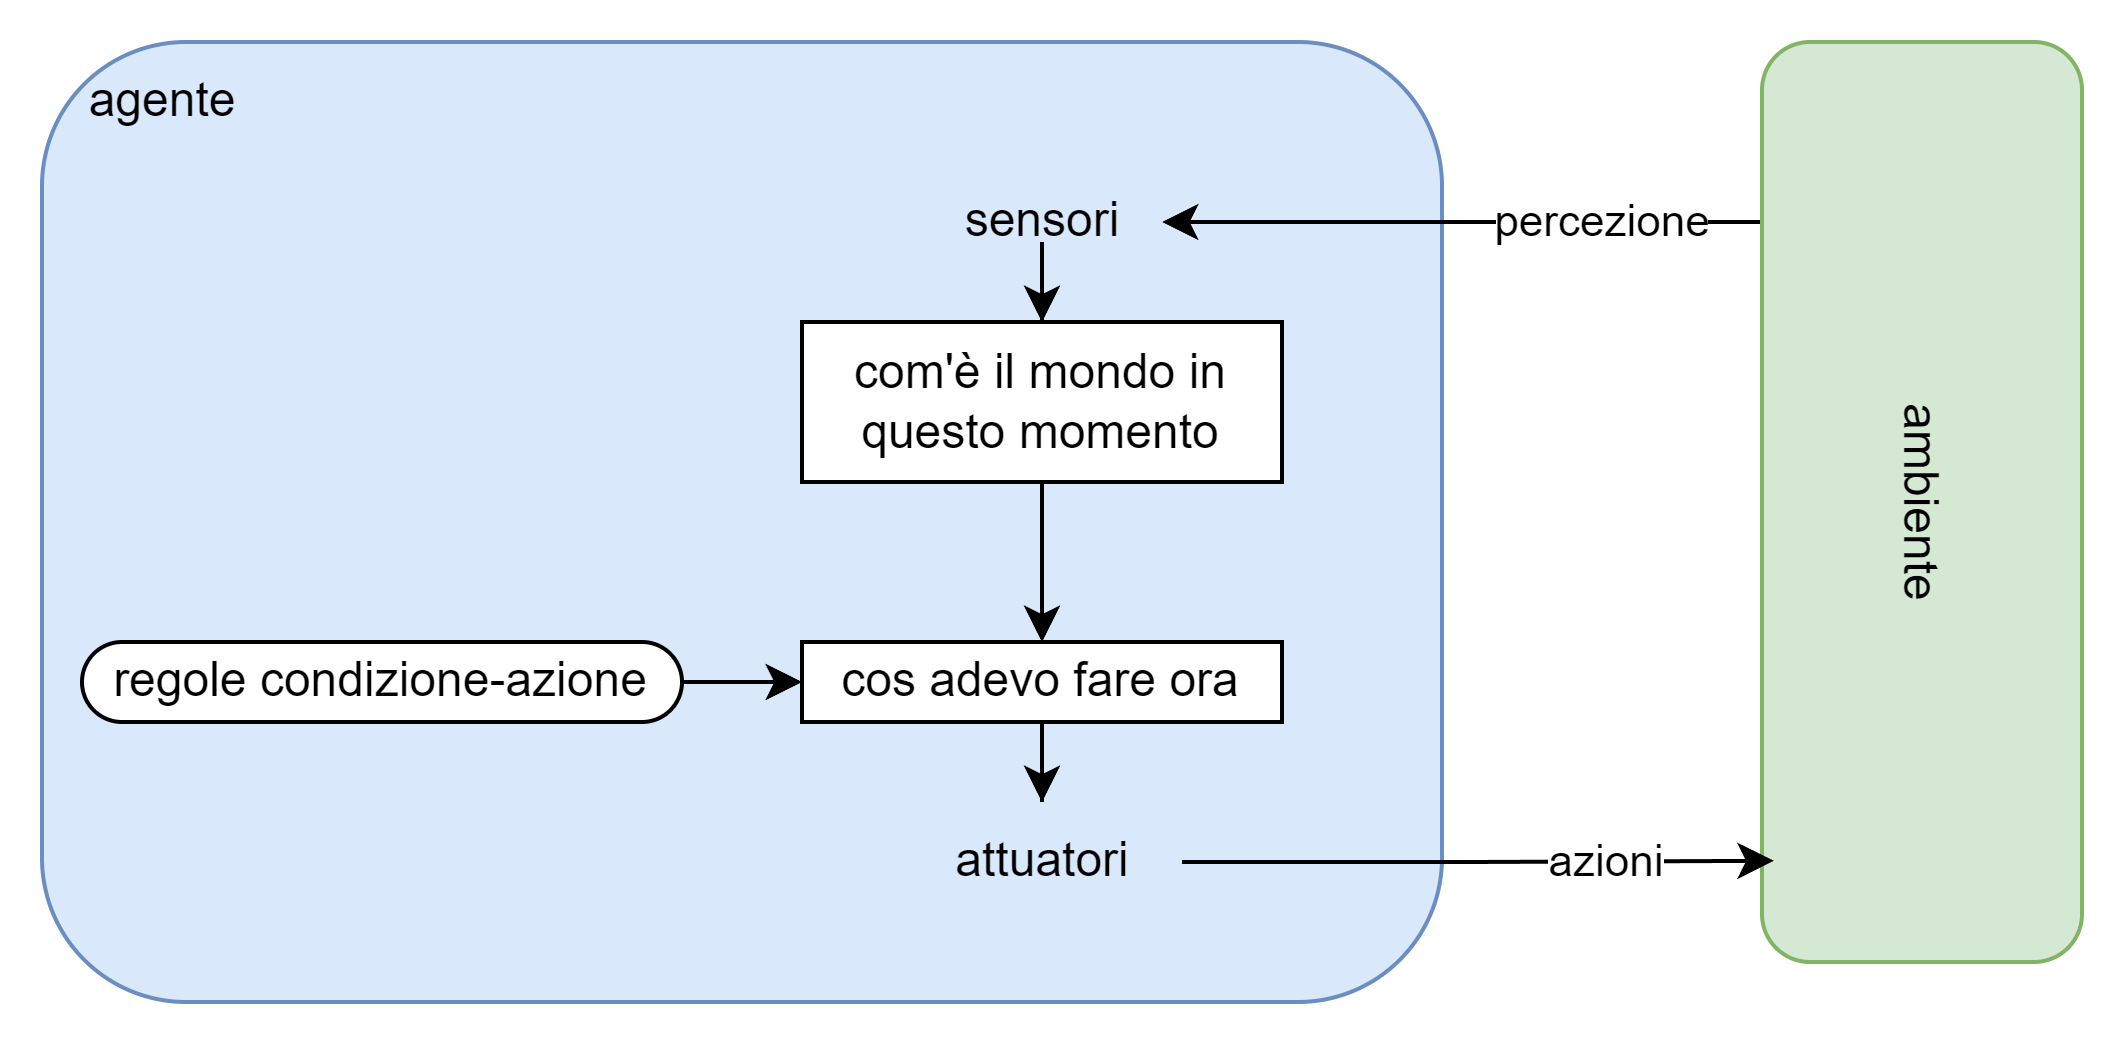
\includegraphics[width=0.8\textwidth]{capitoli/agenti-intelligenti/imgs/simple-reflex.png}
\end{figure}

\begin{lstlisting}
	function SIMPLE-REFLEX-AGENT(percept) returns an action
		persistent: rules, a set of condition-action rules
		
		state = INTERPRET-INPUT(percept)
		rule = RULE-MATCH(state, rules)
		action = rule.ACTION
		return action
\end{lstlisting}

\subsection{\foreignlanguage{english}{Model based reflex agent}}

La maniera più efficiente che l'agente ha per gestire la parziale osservabilità dell'ambiente è quella di tenere traccia della porzione di mondo che non può vedere in questo istante.

L'agente deve mantenere uno stato interno che dipende sulla storia delle percezioni e riflette almeno uno degli aspetti non osservabili dello stato attuale.

Per aggiornare lo stato interno dell'agente al passare del tempo abbiamo bisogno d'inserire due tipi di conoscenza nel programma agente:

\begin{itemize}
	\item informazione su come il mondo cambia nel tempo, che può essere suddivisa in:
	\begin{itemize}
		\item gli effetti delle azioni dell'agente 
		\item come il mondo evolve indipendentemente dall'agente → modello di transizione
	\end{itemize}
	\item informazione su come lo stato dell'ambiente si riflette sulle percezioni dell'agente → modello del sensore
\end{itemize}

Modello di transizione e modello del sensore permettono all'agente di tenere traccia dello stato del mondo. Un agente che usa questi modelli è detto \foreignlanguage{english}{Model based agent}.

\begin{figure}[H]
	\centering
	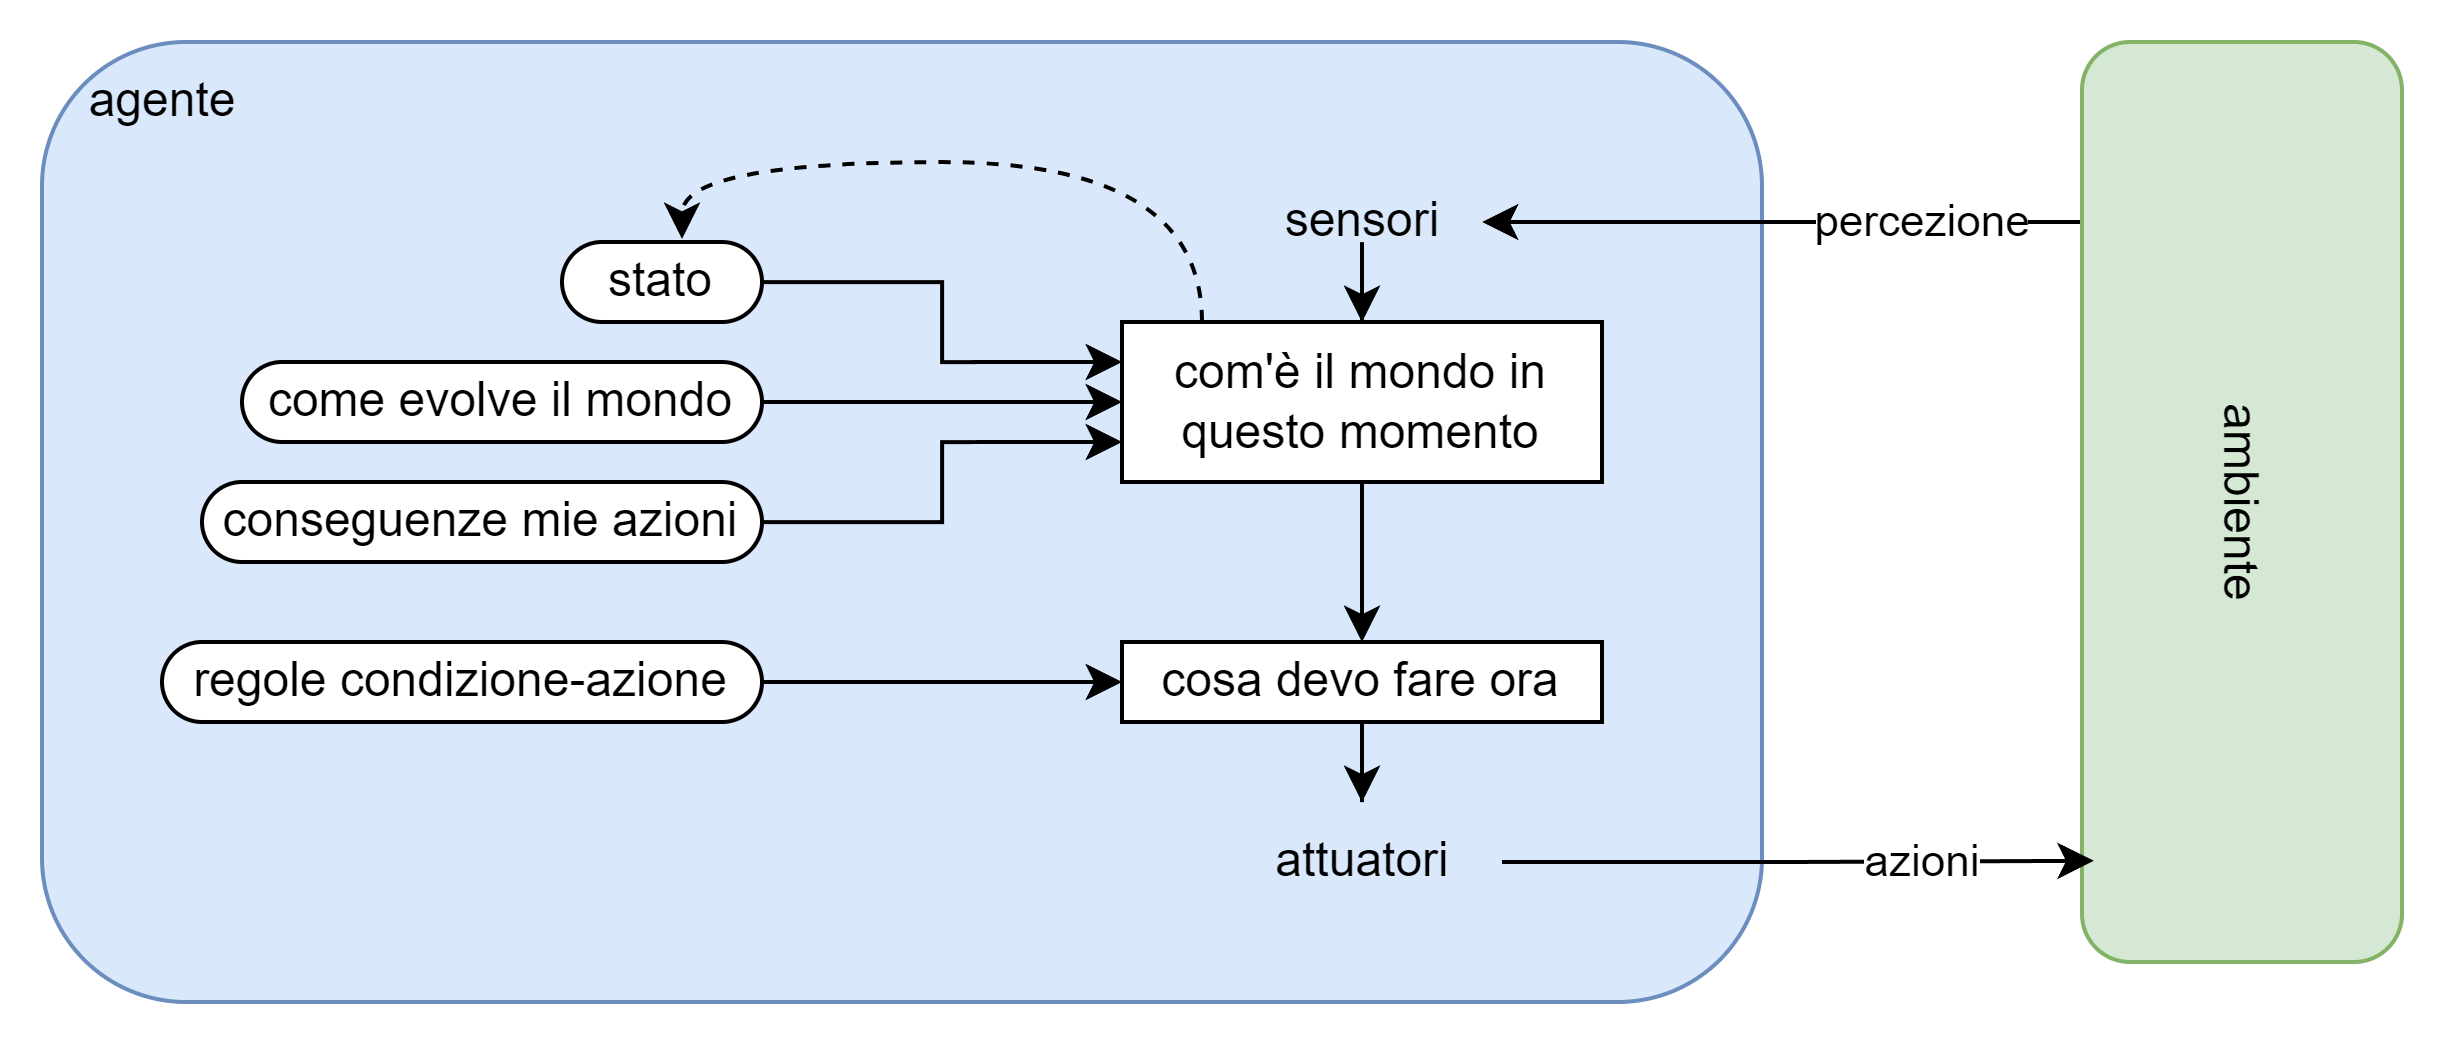
\includegraphics[width=0.8\textwidth]{capitoli/agenti-intelligenti/imgs/model-based.png}
\end{figure}

Nella figura vediamo che la percezione attuale viene combinato con lo stato interno precedente per generare una descrizione aggiornata dello stato corrente, basato sul modello del funzionamento del mondo (1b).

\begin{lstlisting}
	function MODEL-BASED-REFLEX-AGENT(percept) returns an action
		persistent: (state, transition_model, sensor_model, rules, action)
		state = UPDATE-STATE(state, action, percept, transition_model, sensor_model)
		rule = RULE-MATCH(state, rules)
		action = rule.ACTION
		return action
\end{lstlisting}

La funzione UPDATE-STATE è responsabile della creazione del nuovo stato interno.

Raramente un agente riesce a determinare lo stato corrente di un mondo parzialmente osservabile, può lavorare solo sulla migliore approssimazione.

\subsection{\foreignlanguage{english}{Goal based agent}}

Insieme alla descrizione dello stato corrente, l'agente ha bisogno di qualche tipo d'informazione sul suo obiettivo che descriva la situazione desiderabile.

Questo tipo di agente è più flessibile perché la conoscenza che supporta le sue decisioni è rappresentata esplicitamente e può essere modificata.

\begin{figure}[H]
	\centering
	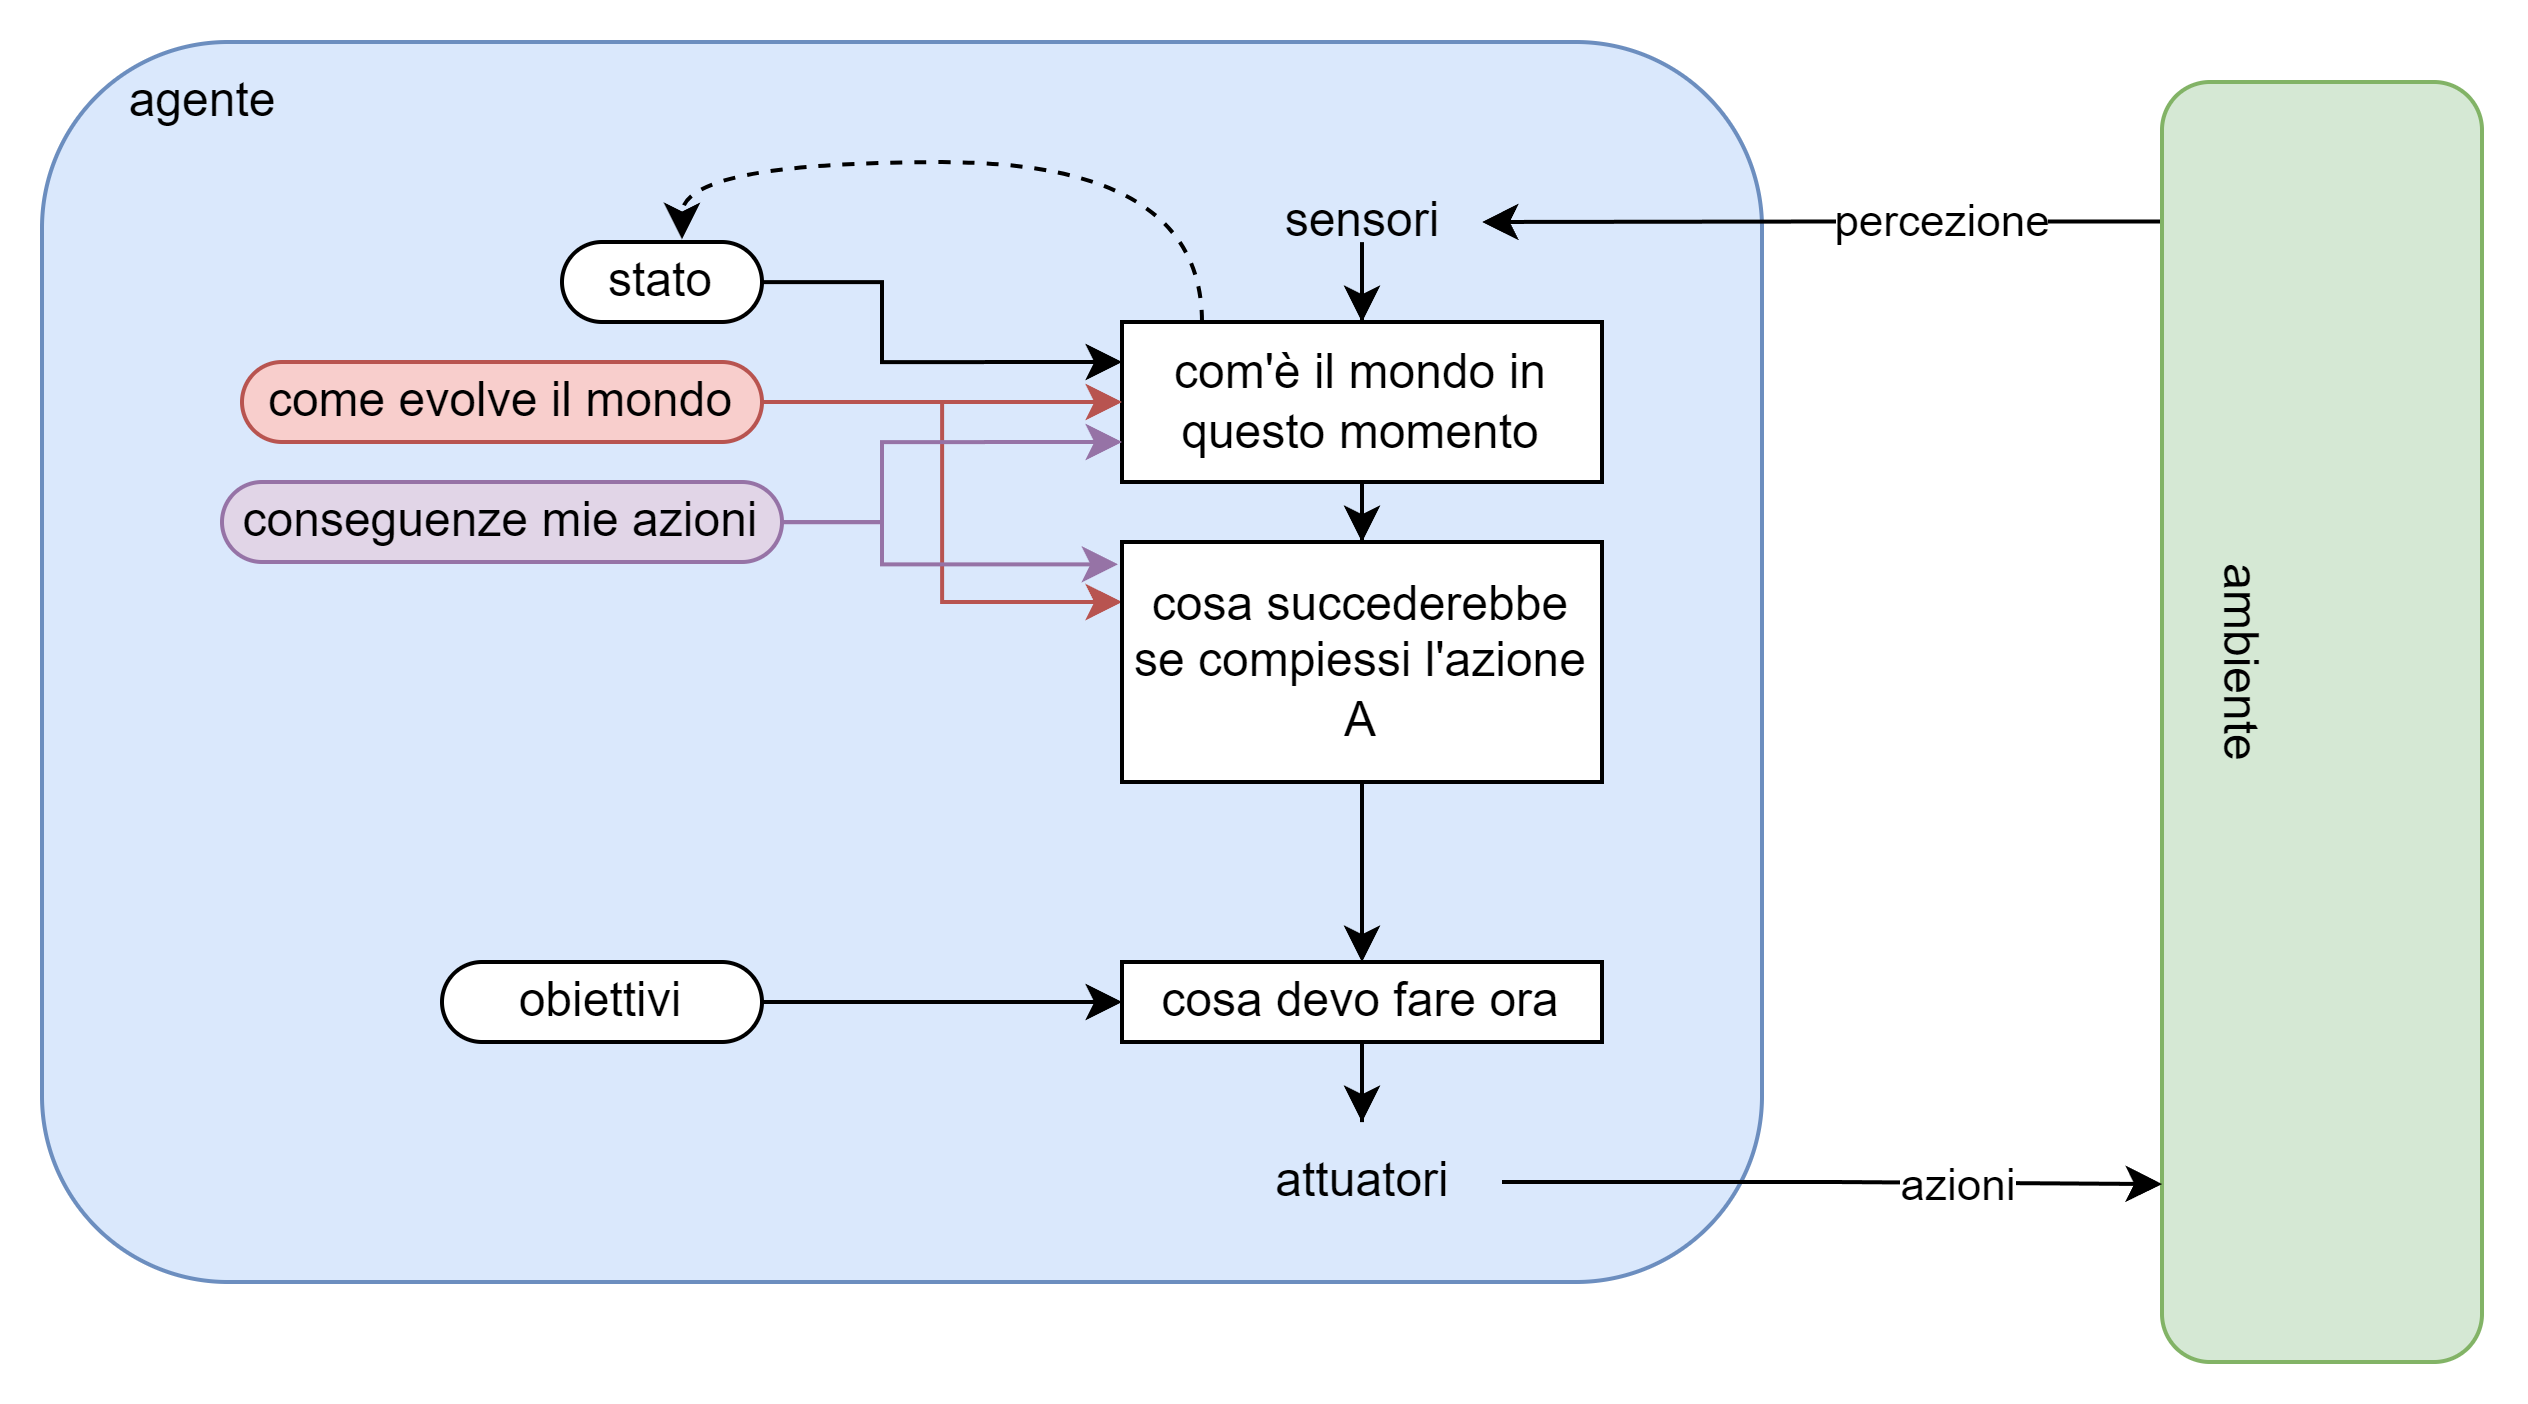
\includegraphics[width=0.8\textwidth]{capitoli/agenti-intelligenti/imgs/goal-based.png}
\end{figure}

\subsection{\foreignlanguage{english}{Utility based agents}}

Gli obiettivi da soli non sono sufficienti a generare un comportamento di alta qualità nella maggior parte degli ambienti.

Gli obiettivi forniscono solo una differenziazione tra “utile” e “non utile”. Ma una misurazione delle performance più accurata prende in considerazione anche la quantità di utile ottenuto.

La misurazione delle performance assegna un punteggio a ogni sequenza di stati dell'ambiente, quindi possiamo distinguere tra i modi più o meno desiderabili di raggiungere l'obiettivo.

La funzione di utilità dell'agente è un'interiorizzazione della misurazione delle performance.
Dal momento che la funzione di utilità e la misurazione delle performance sono allineate, un agente che sceglie azioni che massimizzano la sua utilità sarà giudicato razionale in accordo con la misurazione delle performance.

La funzione di utilità aiuta anche a scegliere quale compromesso adottare, si sceglie quello con maggiore utilità. Nel momento in cui ci sono più obiettivi che l'agente può completare, la funzione di utilità fornisce un mezzo per pesarne la possibilità di successo.

Un agente di questo tipo sceglie l'azione che massimizza l'utilità attesa delle conseguenze dell'azione.

\begin{figure}[H]
	\centering
	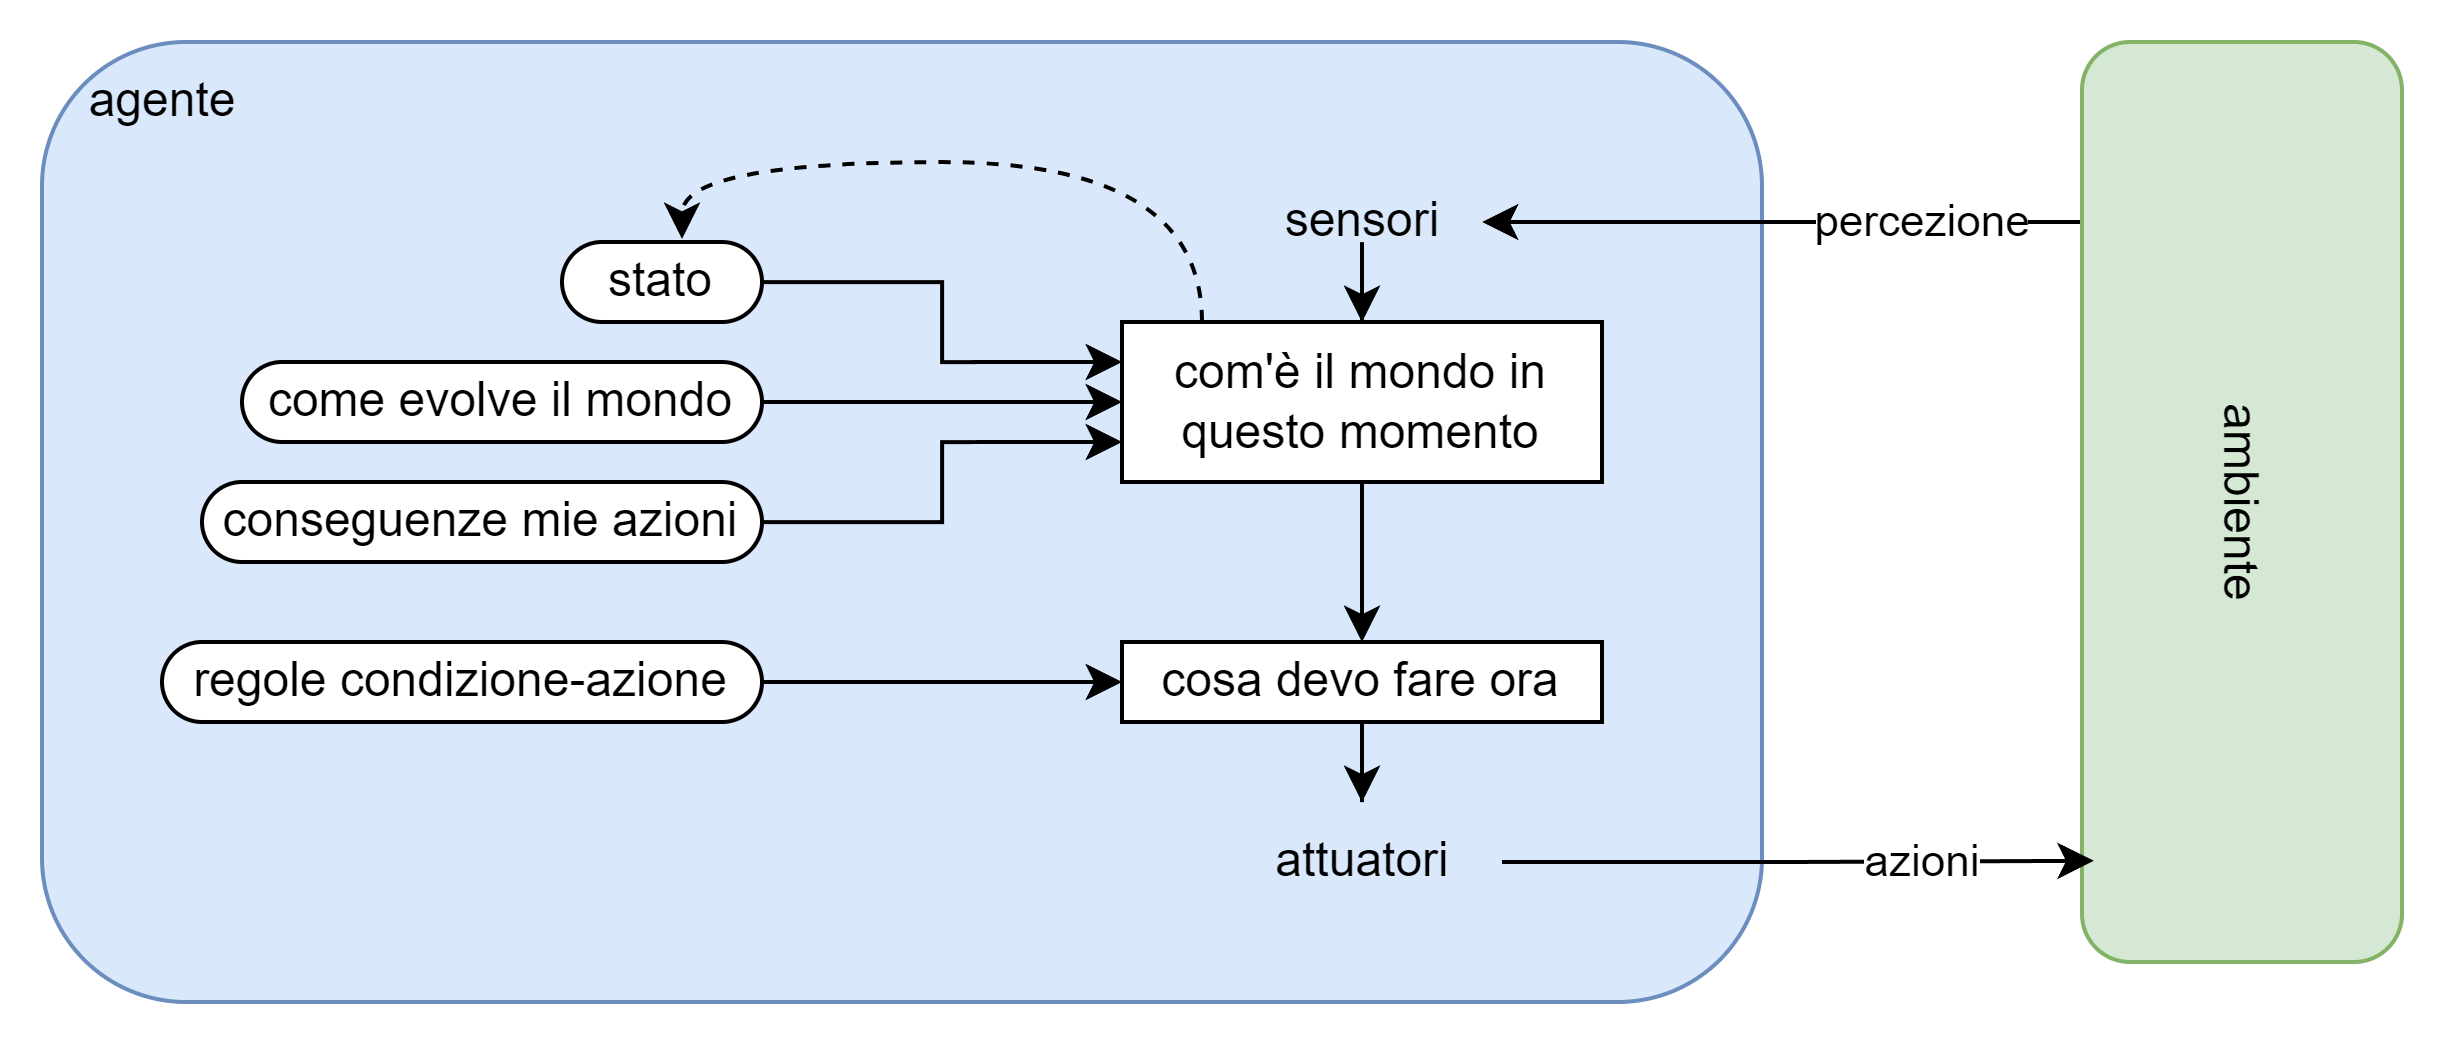
\includegraphics[width=0.8\textwidth]{capitoli/agenti-intelligenti/imgs/model-based.png}
\end{figure}

\subsection{\foreignlanguage{english}{Learning agents}}

L'apprendimento permette all'agente di operare in un ambiente inizialmente sconosciuto e di diventare più competente di quanto la sua conoscenza iniziale gli permetta.

\begin{figure}[H]
	\centering
	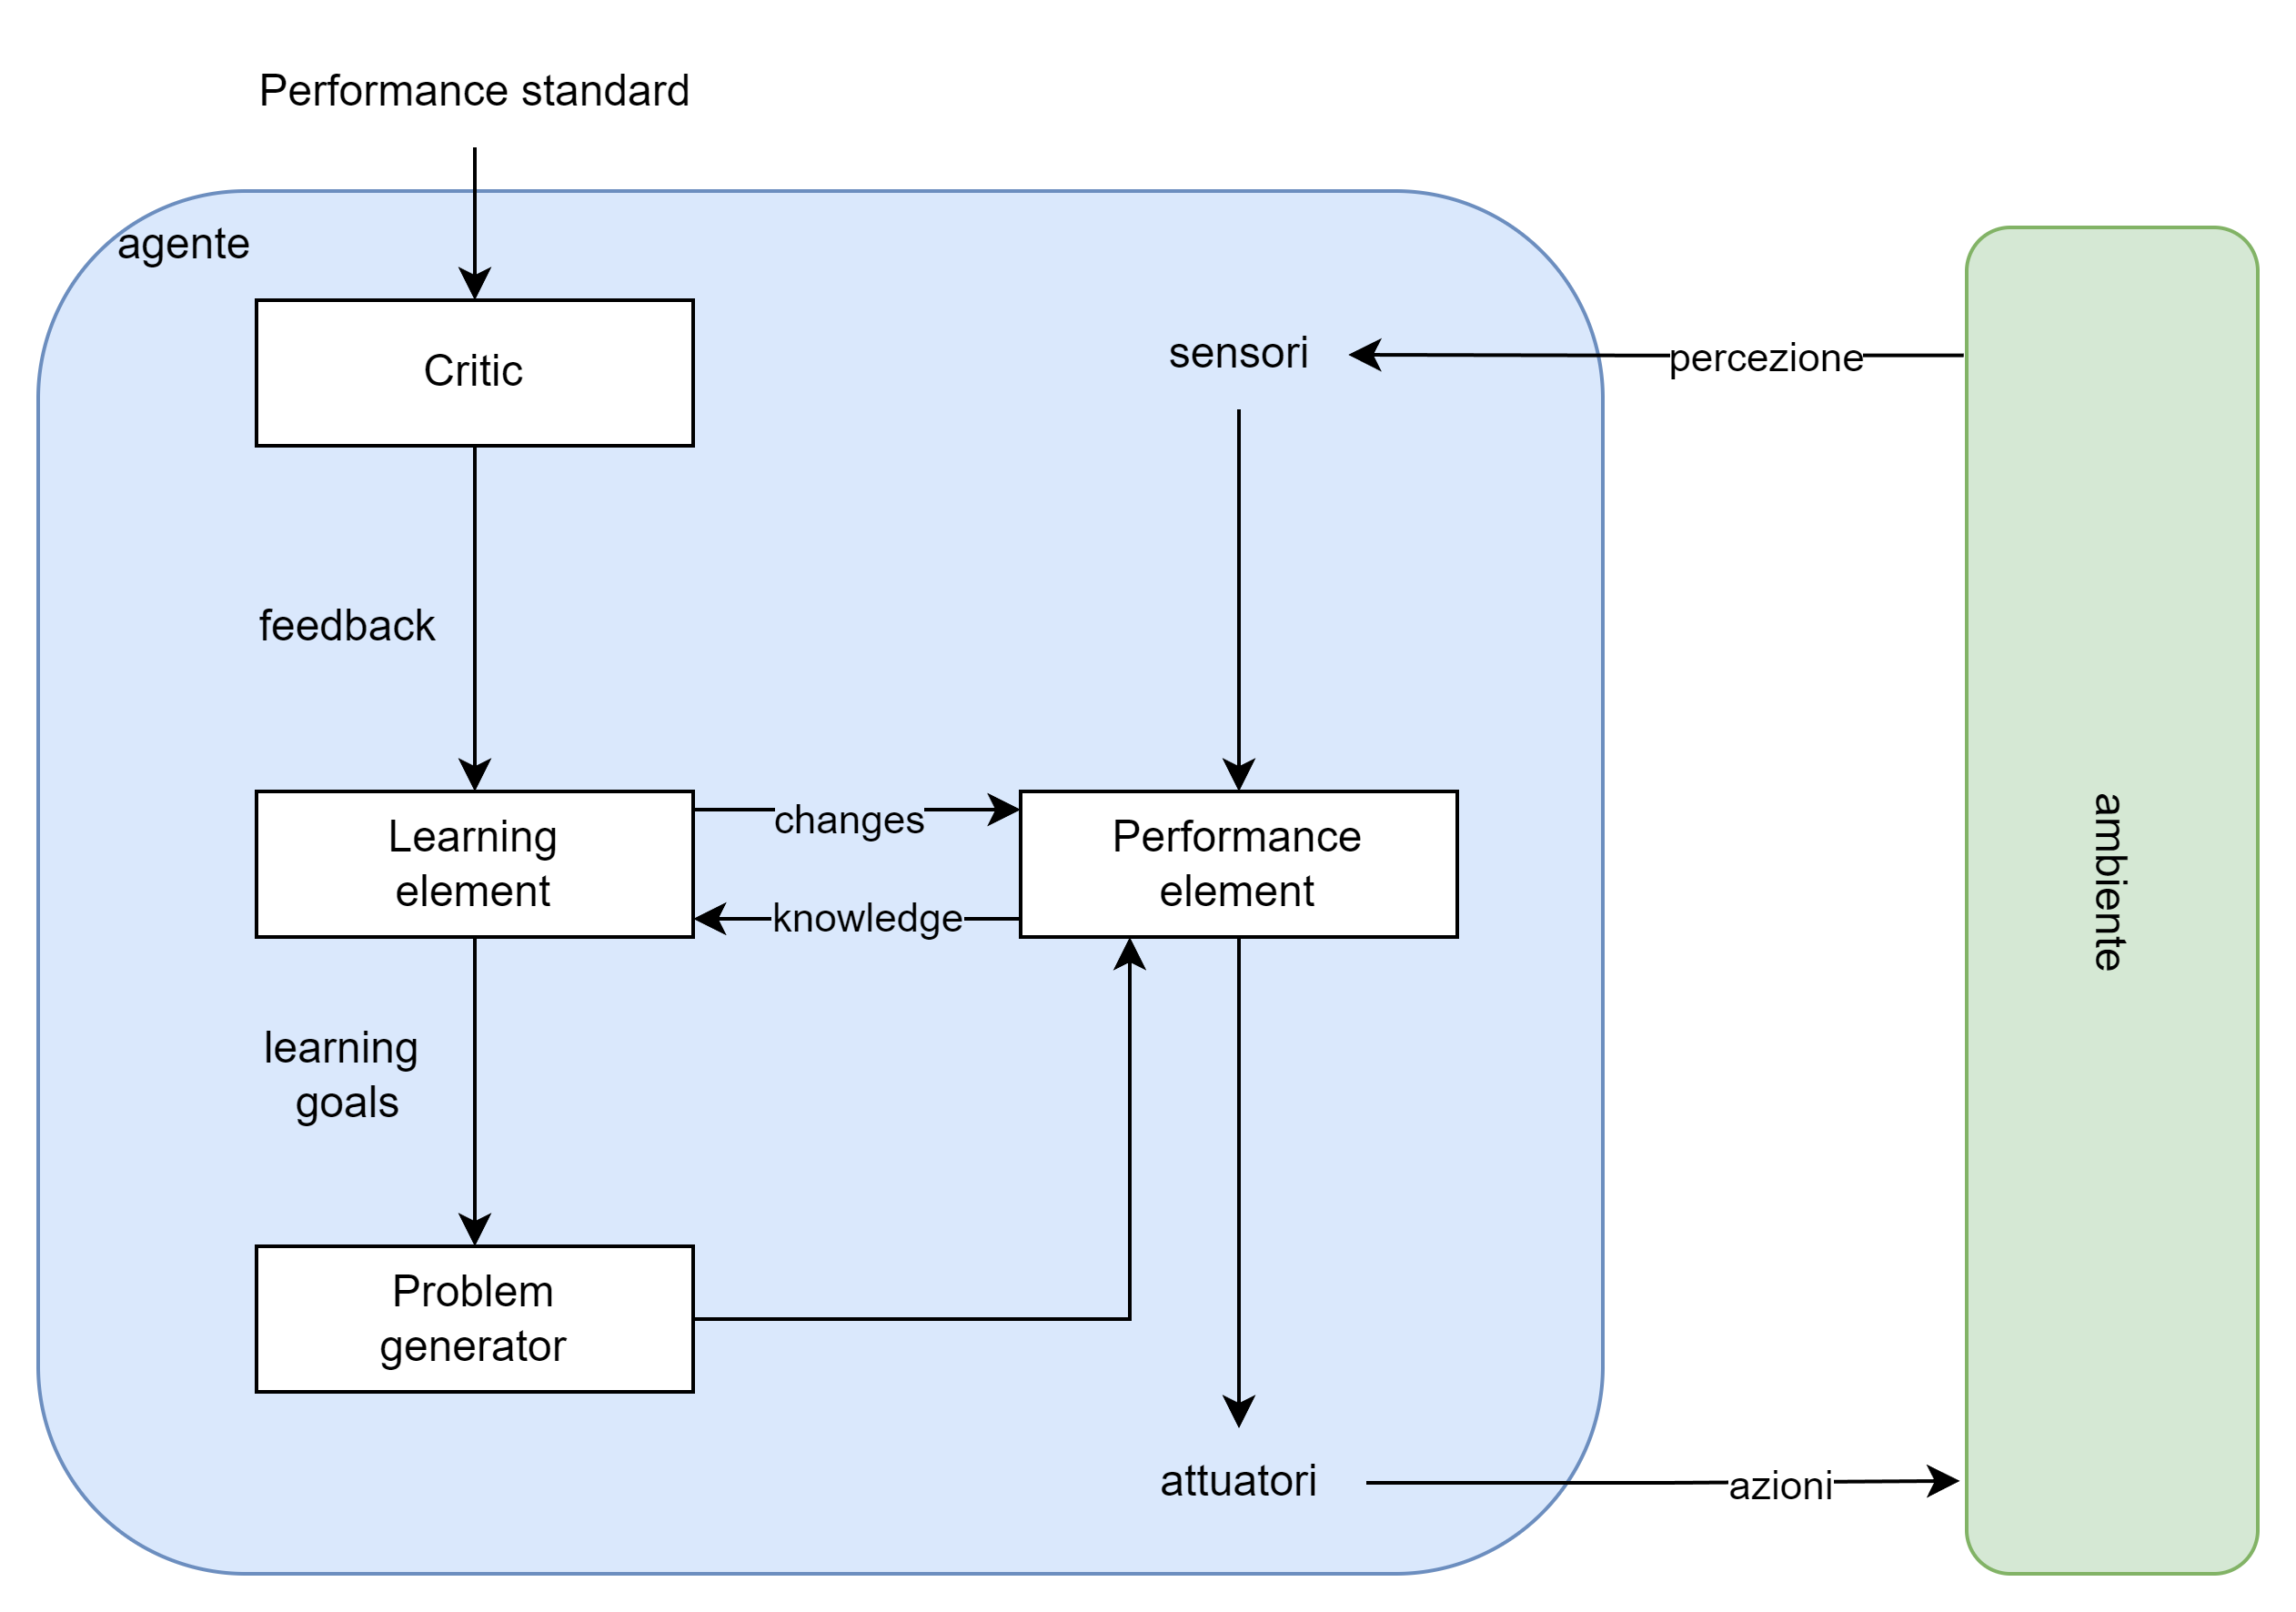
\includegraphics[width=0.8\textwidth]{capitoli/agenti-intelligenti/imgs/learning.png}
\end{figure}

Un agente che apprende può essere suddiviso in quattro componenti concettuali:

\begin{itemize}
	\item Elemento di apprendimento: responsabile degli avanzamenti fatti, ottiene feedback dalla critica su come l'agente si sta comportando e determina come l'elemento di performance deve essere modificato per fare meglio in futuro
	\item elemento di performance: quello che nei precedenti modelli era l'intero agente, prende in ingresso le percezioni e restituisce le azioni
	\item critica: fornisce feedback sul successo delle azioni dell'agente
	\item generatore di problemi: suggerisce azioni che poteranno a nuove esperienze, suggerisce azioni di esplorazione. Potrebbe identificare parti del modello che hanno bisogno di miglioramenti e suggerire esperimenti.
\end{itemize}

L'apprendimento può essere riassunto come il processo di modificazione di ogni componente dell'agente per fare in modo che essi siano più in linea con il feedback esterno, migliorando le performance complessive dell'agente.

\subsection{Come funzionano i componenti degli agenti}

Un componente può rappresentare il mondo che lo circonda in maniera:

\begin{itemize}
	\item atomica
	\item fattorizzata
	\item strutturata
\end{itemize}

\begin{figure}[H]
	\centering
	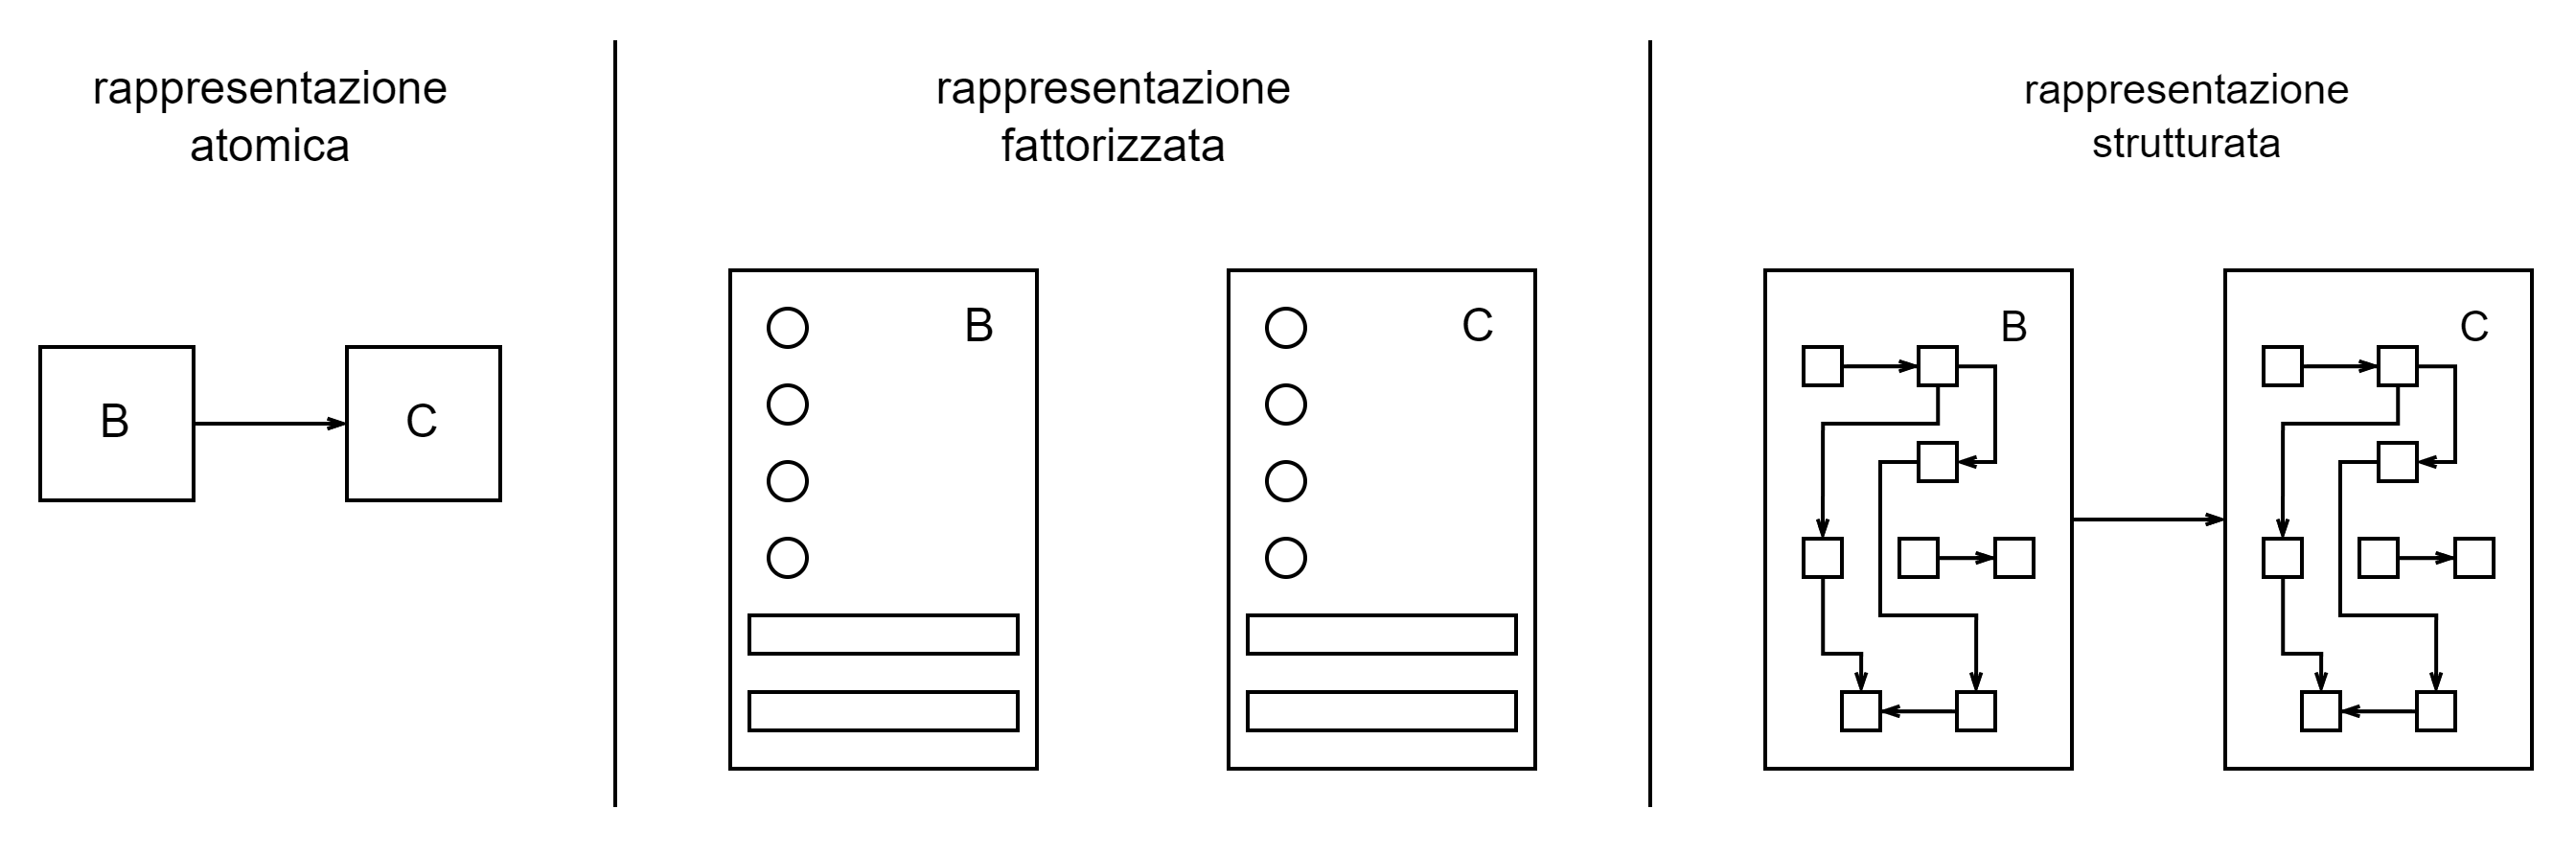
\includegraphics[width=0.8\textwidth]{capitoli/agenti-intelligenti/imgs/componenti.png}
\end{figure}

Nella rappresentazione atomica ogni stato è indivisibile, è trattato come una scatola nera. Due stati atomici non hanno nulla in comune, li distingue l'unica informazione che contengono.

Nella rappresentazione fattorizzata ogni stato è suddiviso in un insieme fissato di variabili e attributi con un proprio valore. Due stati in questa rappresentazione possono condividere il valore di alcune variabili.

Nella rappresentazione strutturata gli stati contengono oggetti in relazione tra loro.

Le rappresentazioni elencate vanno dalla meno alla più rappresentativa. 
Con l'aumento dell'espressività aumenta anche la difficoltà di apprendimento 
quindi gli agenti intelligenti hanno bisogno di operare con diverse 
rappresentazioni simultaneamente.

Un'altra distinzione che possiamo fare riguardo al funzionamento del componente è basata sulla locazione delle informazioni; possiamo distinguere tra rappresentazioni localizzate, in cui esiste una mappatura 1-a-1 tra un concetto e una locazione di memoria, e rappresentazioni distribuite, in cui la rappresentazione di un concetto è distribuita in più locazioni.